\appendix

\chapter{Map figures used in both versions of the questionnaire}
\label{appendix:a}

\begin{figure}[h]
    \caption{Maps used in the questionnaires}
    \centerline{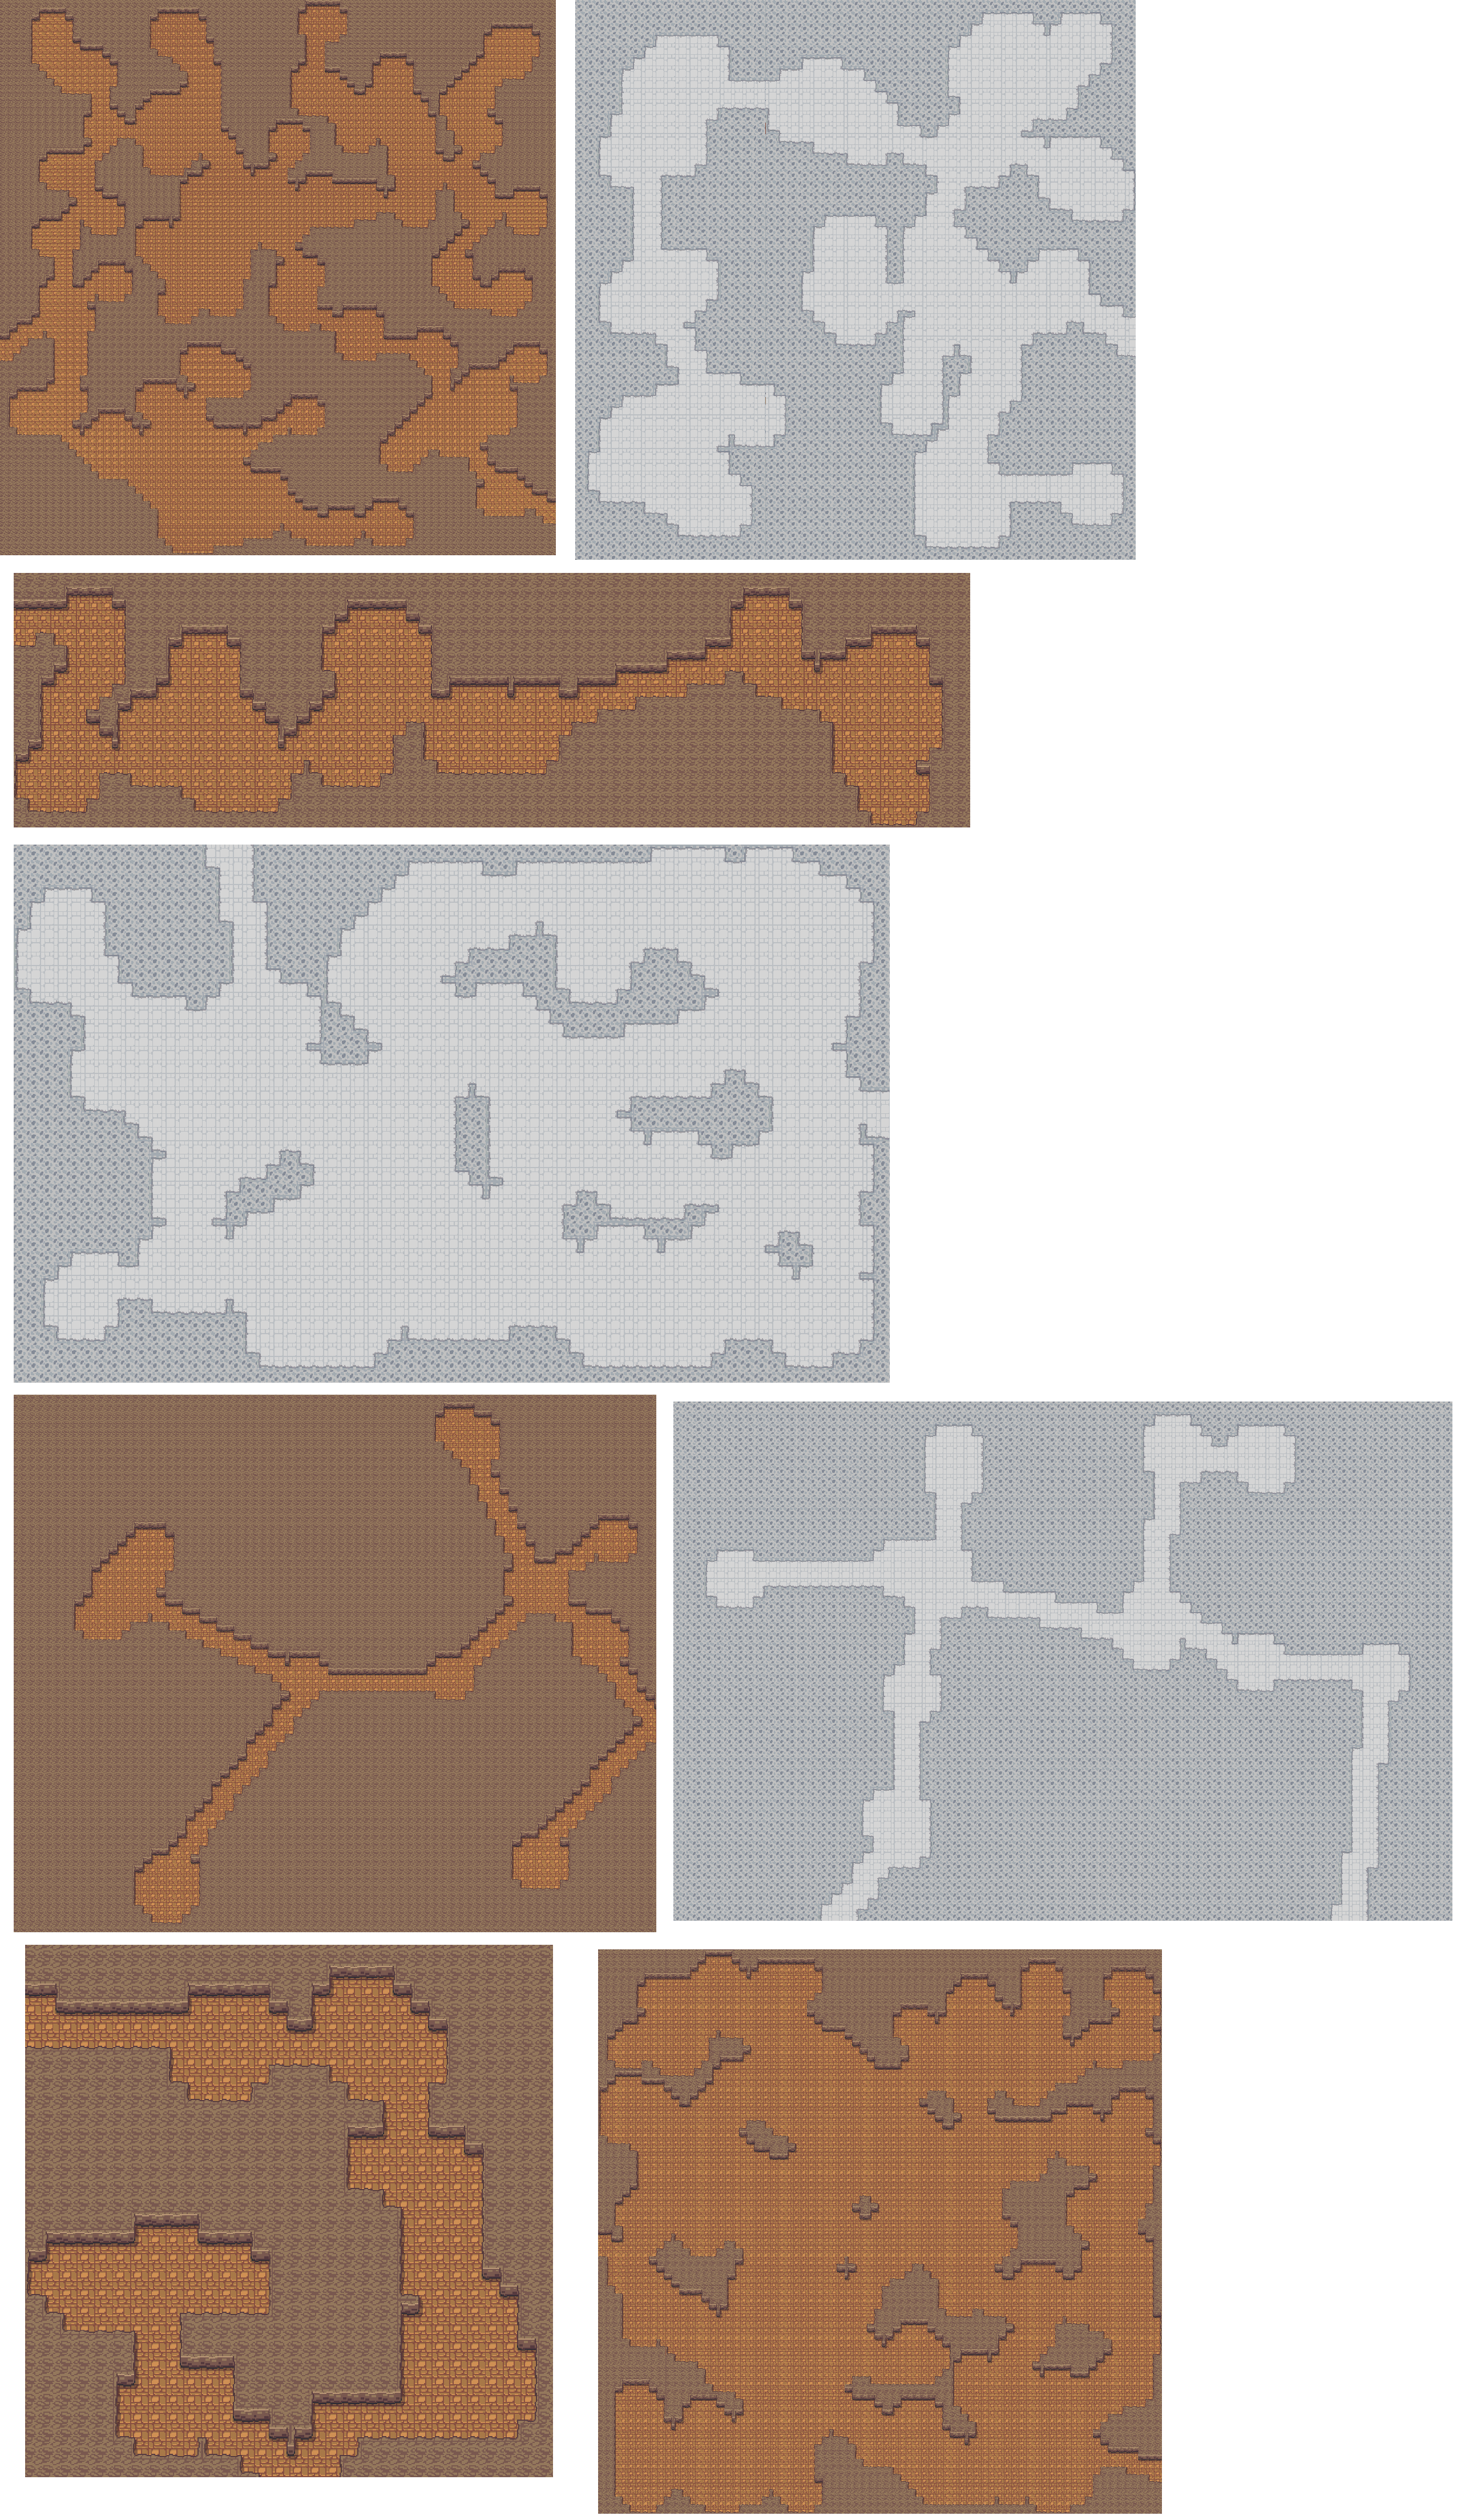
\includegraphics[width=10.505cm]{images/survey/allmaps.png}}
    \legend{Source: Image provided by author}
\end{figure}

\chapter{Pretest questionnaire}
\label{appendix:b}

\begin{table}[h]
\caption{Part of the pretest questionnaire regarding the maps.}
\resizebox{\textwidth}{!}{%
\begin{tabular}{|l|l|l|}
\hline
No. & Question & Justification \\ \hline
1 & \begin{tabular}[c]{@{}l@{}}There was something interesting in the cave \\ maps that caught my attention.\end{tabular} & \begin{tabular}[c]{@{}l@{}}Question related to the Attention component of the \\ ARCS model.\end{tabular} \\ \hline
2 & \begin{tabular}[c]{@{}l@{}}The first time I saw the cave maps, I had the \\ impression that they would be easy to explore.\end{tabular} & \begin{tabular}[c]{@{}l@{}}Question related to the Confidence component of \\ the ARCS model.\end{tabular} \\ \hline
3 & \begin{tabular}[c]{@{}l@{}}The structure of the caves was harder to \\ comprehend than I would have liked them to be.\end{tabular} & \begin{tabular}[c]{@{}l@{}}Question related to the Confidence component of\\ the ARCS model.\end{tabular} \\ \hline
4 & \begin{tabular}[c]{@{}l@{}}While looking at the maps, I feel that it would\\  be easy for me to get lost.\end{tabular} & \begin{tabular}[c]{@{}l@{}}Question related to the criteria: maps should have\\ \\ an entrance, an exit, and a path between them.\end{tabular} \\ \hline
5 & \begin{tabular}[c]{@{}l@{}}The structure of the map looked natural, it didn't \\ look like it was generated by an algorithm.\end{tabular} & \begin{tabular}[c]{@{}l@{}}Question related to the criteria: generated maps\\ should have a natural look.\end{tabular} \\ \hline
6 & \begin{tabular}[c]{@{}l@{}}While I observed the maps, I felt like I was\\ seeing a representation of real caves.\end{tabular} & \begin{tabular}[c]{@{}l@{}}Question related to the criteria: generated maps\\ should have a natural look.\end{tabular} \\ \hline
7 & \begin{tabular}[c]{@{}l@{}}In the generated maps, what reminds me of a \\ real cave are the used colors, and not the \\ structure of paths.\end{tabular} & \begin{tabular}[c]{@{}l@{}}This question serves to evaluate how important\\ the structure is in the creation of a natural look.\end{tabular} \\ \hline
8 & \begin{tabular}[c]{@{}l@{}}In the generated maps, what reminds me of a\\ real cave is the structure of paths, and not the\\ used colors.\end{tabular} & \begin{tabular}[c]{@{}l@{}}This question serves to evaluate how important\\ the used colors are in the creation of a natural look.\end{tabular} \\ \hline
9 & \begin{tabular}[c]{@{}l@{}}The generated map's design made it difficult \\ for me to keep my attention.\end{tabular} & \begin{tabular}[c]{@{}l@{}}Question related to the Attention component of \\ the ARCS model.\end{tabular} \\ \hline
10 & \begin{tabular}[c]{@{}l@{}}The generated cave maps were capable of\\ capturing my attention.\end{tabular} & \begin{tabular}[c]{@{}l@{}}Question related to the Attention component of\\ the ARCS model.\end{tabular} \\ \hline
11 & \begin{tabular}[c]{@{}l@{}}While looking at the maps, I feel like exploring\\ them.\end{tabular} & \begin{tabular}[c]{@{}l@{}}Question related to the criteria: maps should\\ encourage players to explore.\end{tabular} \\ \hline
12 & \begin{tabular}[c]{@{}l@{}}The design of the generated cave maps is \\ attractive.\end{tabular} & \begin{tabular}[c]{@{}l@{}}This question serves to evaluate the overall\\ attractiveness of the maps.\end{tabular} \\ \hline
13 & \begin{tabular}[c]{@{}l@{}}The design of the maps is very simple and not\\ attractive.\end{tabular} & \begin{tabular}[c]{@{}l@{}}This question serves to evaluate the overall \\ attractiveness of the design.\end{tabular} \\ \hline
14 & \begin{tabular}[c]{@{}l@{}}The generated structures look very similar,\\ with little variety.\end{tabular} & \begin{tabular}[c]{@{}l@{}}Question related to the criteria: maps should\\ look different from one another\end{tabular} \\ \hline
15 & \begin{tabular}[c]{@{}l@{}}The variety of the maps helps to keep my\\ attention.\end{tabular} & \begin{tabular}[c]{@{}l@{}}Question related to the criteria: maps should\\ look different from one another.\end{tabular} \\ \hline
\end{tabular}%
}
\legend{Source: Table provided by author.}
\end{table}

\begin{table}[H]
\caption{Part of the pretest questionnaire regarding the questionnaire itself.}
\resizebox{\textwidth}{!}{%
\begin{tabular}{|l|l|}
\hline
No. & Question \\ \hline
1 & Do you think that the questions from this questionnaire were easy to understand? If not, why? \\ \hline
2 & Are there repeated questions in this questionnaire? If yes, which? \\ \hline
3 & Would you include other questions on this questionnaire? If yes, which? \\ \hline
4 & Would you change the text of one or more questions in this questionnaire? If yes, which? \\ \hline
5 & \begin{tabular}[c]{@{}l@{}}Do you think a question comparing the generated maps to real cave representation is necessary \\ for this questionnaire?\end{tabular} \\ \hline
\end{tabular}%
}
\legend{Source: Table provided by author.}
\label{table:pretest_quest}
\end{table}

\chapter{Second version of the questionnaire}
\label{appendix:c}

% Please add the following required packages to your document preamble:
% \usepackage{graphicx}
\begin{table}[h]
\caption{Second version of the questionnaire.}
\resizebox{\textwidth}{!}{%
\begin{tabular}{|l|l|l|}
\hline
No. & Question & Justification \\ \hline
1 & \begin{tabular}[c]{@{}l@{}}There was something interesting in the cave \\ maps that caught my attention.\end{tabular} & \begin{tabular}[c]{@{}l@{}}Question related to the Attention component of the \\ ARCS model.\end{tabular} \\ \hline
2 & \begin{tabular}[c]{@{}l@{}}The structure of the caves was harder to \\ comprehend than I would have liked them to be.\end{tabular} & \begin{tabular}[c]{@{}l@{}}Question related to the Confidence component of\\ the ARCS model.\end{tabular} \\ \hline
3 & \begin{tabular}[c]{@{}l@{}}I feel like it would be easy for me to get lost in\\ more than one of the observed maps.\end{tabular} & \begin{tabular}[c]{@{}l@{}}Question related to the criteria: maps should have\\ an entrance, an exit, and a path between them.\end{tabular} \\ \hline
4 & \begin{tabular}[c]{@{}l@{}}In more than one of the generated maps, the \\ structure of the map looked natural, it didn't \\ look like it was generated by an algorithm.\end{tabular} & \begin{tabular}[c]{@{}l@{}}Question related to the criteria: generated maps\\ should have a natural look.\end{tabular} \\ \hline
5 & \begin{tabular}[c]{@{}l@{}}While I observed the maps, I felt like I was\\ seeing a representation of real caves.\end{tabular} & \begin{tabular}[c]{@{}l@{}}Question related to the criteria: generated maps\\ should have a natural look.\end{tabular} \\ \hline
6 & \begin{tabular}[c]{@{}l@{}}In the generated maps, what reminds me of a \\ real cave are the used colors and textures.\end{tabular} & \begin{tabular}[c]{@{}l@{}}This question serves to evaluate how important\\ the used colors and textures are in the creation \\ of a natural look.\end{tabular} \\ \hline
7 & \begin{tabular}[c]{@{}l@{}}In the generated maps, what reminds me of a\\ real cave is the structure of paths.\end{tabular} & \begin{tabular}[c]{@{}l@{}}This question serves to evaluate how important\\ the structure of paths are in the creation of a \\ natural look.\end{tabular} \\ \hline
8 & \begin{tabular}[c]{@{}l@{}}The design of more than one map made it \\ difficult for me to keep my attention.\end{tabular} & \begin{tabular}[c]{@{}l@{}}Question related to the Attention component of \\ the ARCS model.\end{tabular} \\ \hline
9 & \begin{tabular}[c]{@{}l@{}}While looking at the maps, I feel like exploring\\ them.\end{tabular} & \begin{tabular}[c]{@{}l@{}}Question related to the criteria: maps should\\ encourage players to explore.\end{tabular} \\ \hline
10 & \begin{tabular}[c]{@{}l@{}}The design of the generated cave maps is \\ attractive.\end{tabular} & \begin{tabular}[c]{@{}l@{}}Question related to the Satisfaction component of\\ the ARCS model.\end{tabular} \\ \hline
11 & \begin{tabular}[c]{@{}l@{}}The generated structures look very similar,\\ with little variety.\end{tabular} & \begin{tabular}[c]{@{}l@{}}Question related to the criteria: maps should\\ look different from one another\end{tabular} \\ \hline
12 & \begin{tabular}[c]{@{}l@{}}I would play a game that utilizes the generated\\ maps.\end{tabular} & \begin{tabular}[c]{@{}l@{}}Question related to the Relevance component of\\ the ARCS model.\end{tabular} \\ \hline
\end{tabular}%
}
\legend{Source: Table provided by author.}
\label{table:final_quest}
\end{table}